\begin{sidewaysfigure}[htbp]
\centering 
  \subfloat%[Jenike shear cell tester.]
  {
	  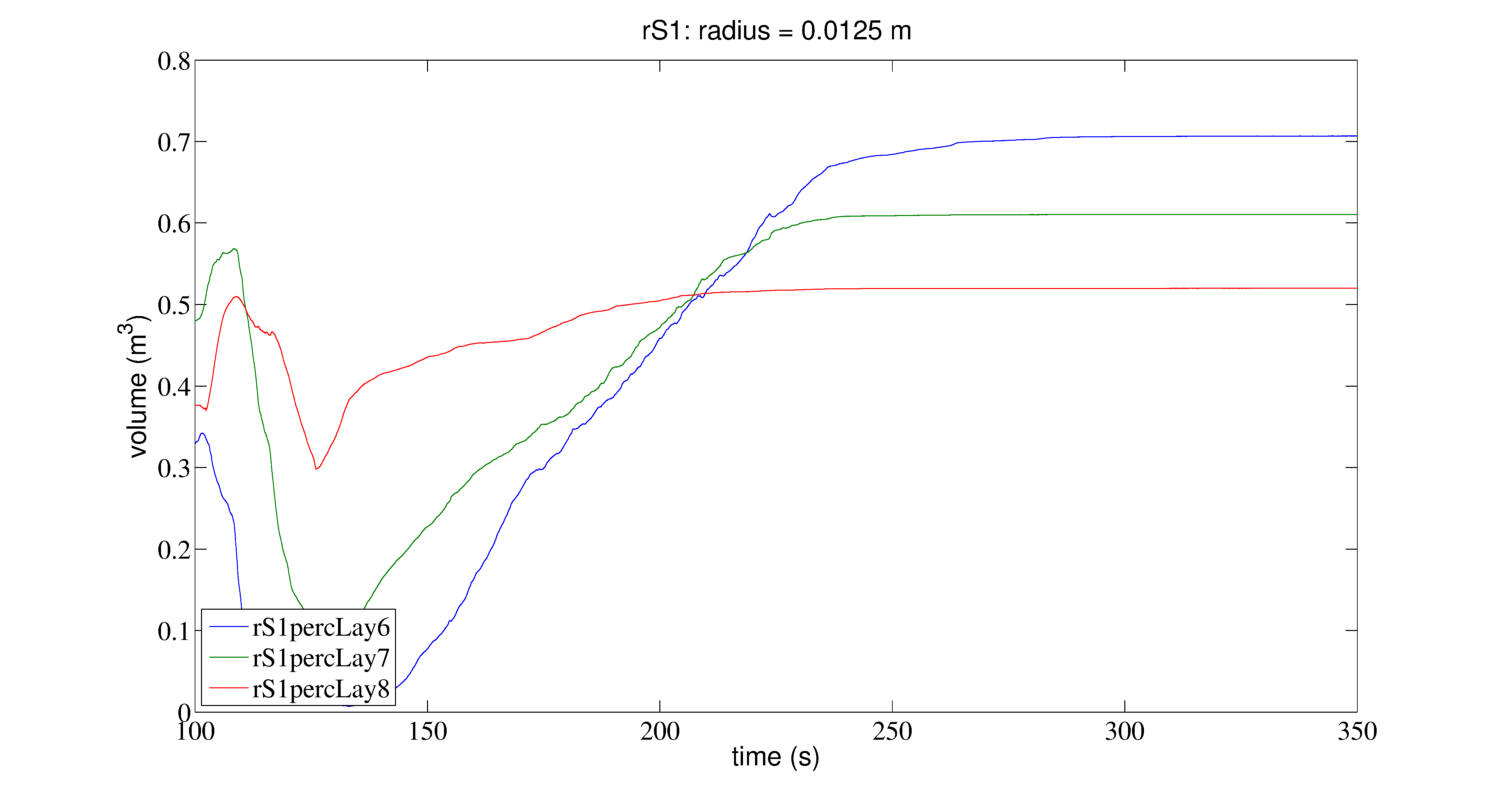
\includegraphics[width=.48\columnwidth]{images/113rS120151111150702}
	  \label{fig:113rS120151111150702}
  }
  \quad
    \subfloat
    %[Simplified Jenike shear cell tester.]
    {
	  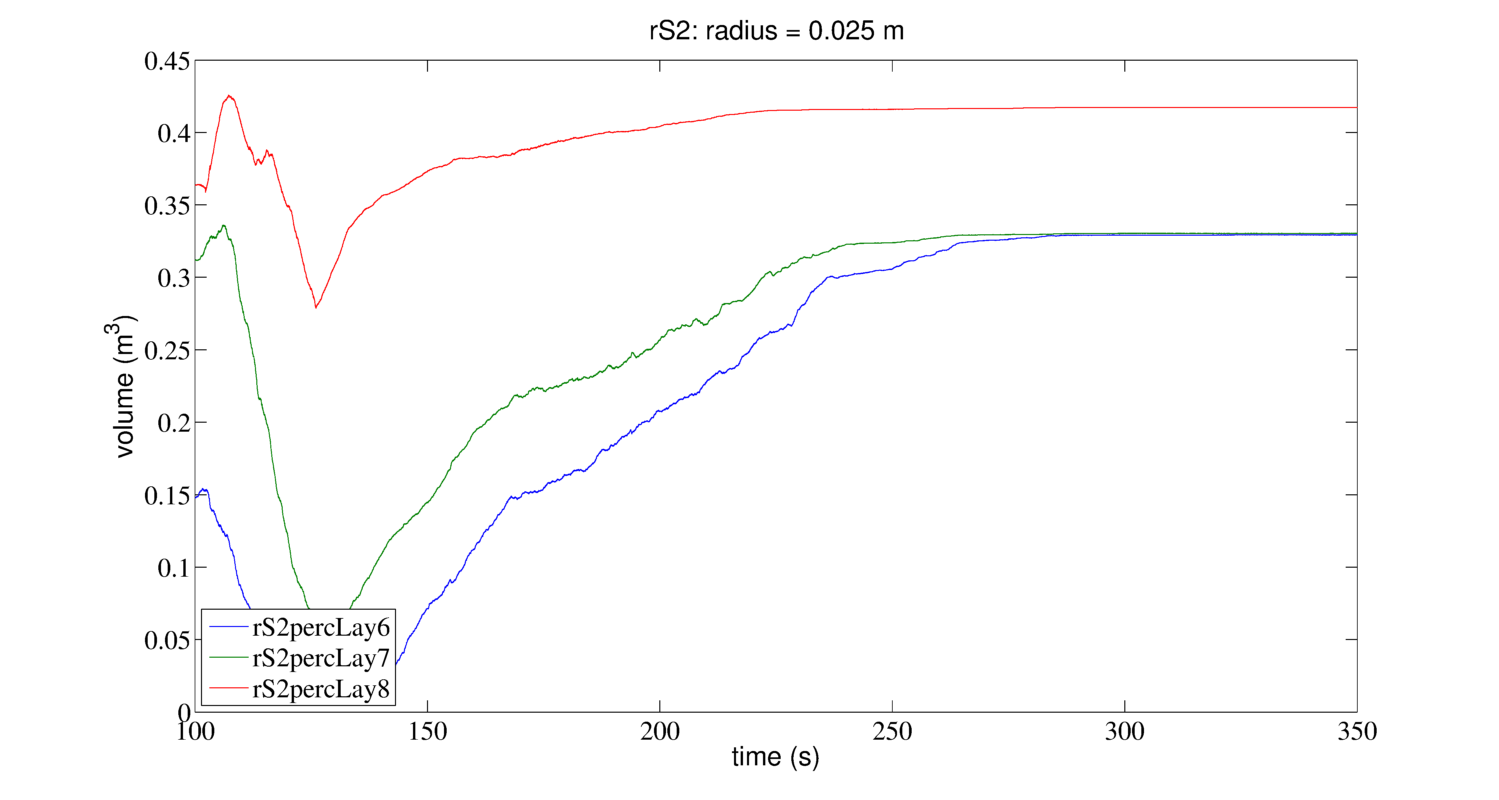
\includegraphics[width=.48\columnwidth]{images/115rS220151111150702}
	  \label{fig:115rS220151111150702}
  }
  \\
  \subfloat%[Jenike shear cell tester layout.]
  {
	  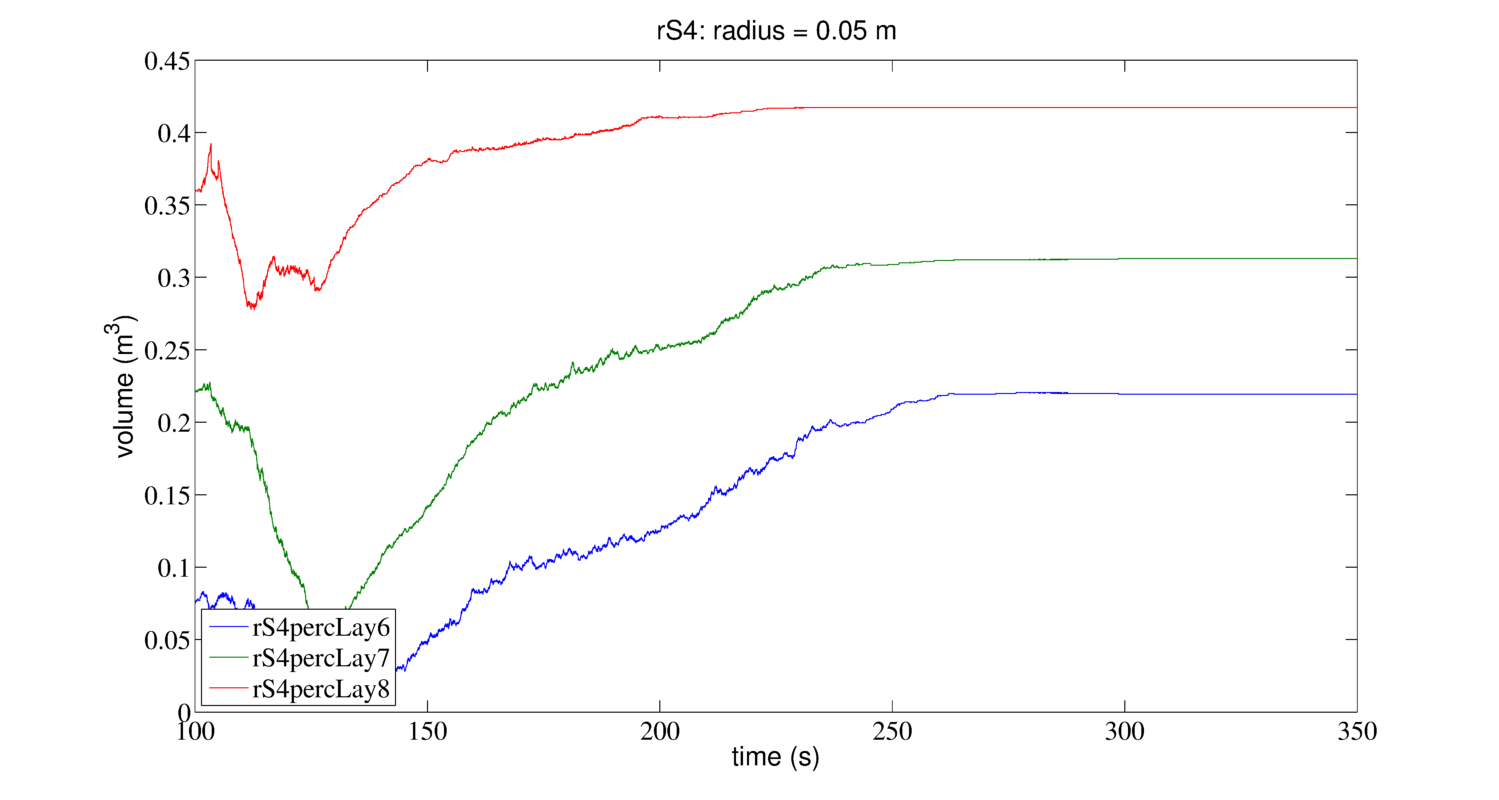
\includegraphics[width=.48\columnwidth]{images/117rS420151111150702}
	  \label{fig:117rS420151111150702}
  }
  \quad
    \subfloat%[Jenike shear cell tester diagram.]
    {
	  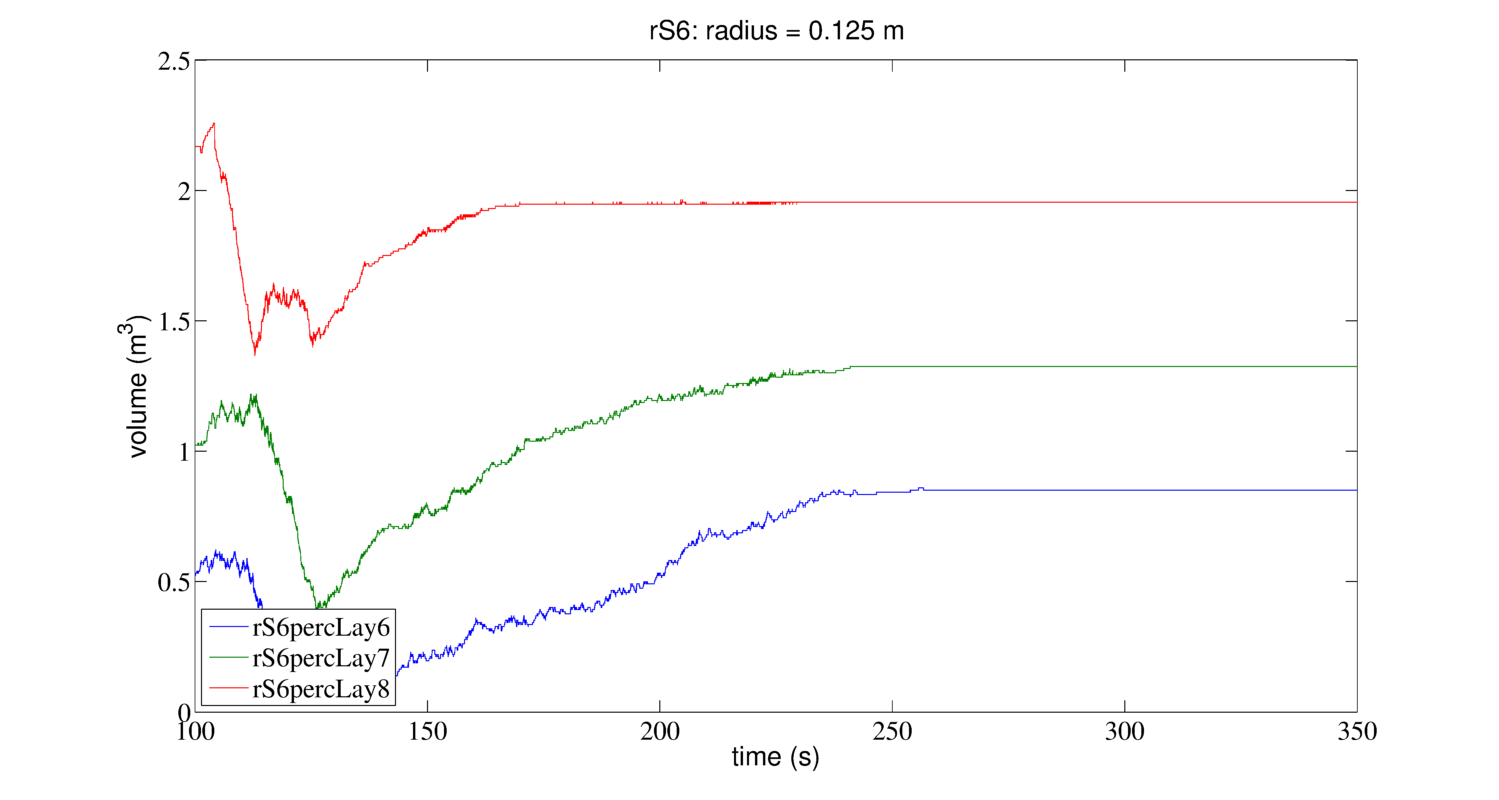
\includegraphics[width=.48\columnwidth]{images/119rS620151111150702}
	  \label{fig:119rS620151111150702}  }
  \\
  \caption[Particle size distribution during the simulation 1]{Particle size
  distribution during the simulation, in $m^3$ of material. Once steady state is
  reached, large particles are more likely in the inferior layers, small particles in the superior ones.}
  \label{fig:096sinterplots}
\end{sidewaysfigure}